%

% File final_report.tex
%
%% Based on the style files for ACL 2020, which were
%% Based on the style files for ACL 2018, NAACL 2018/19, which were
%% Based on the style files for ACL-2015, with some improvements
%%  taken from the NAACL-2016 style
%% Based on the style files for ACL-2014, which were, in turn,
%% based on ACL-2013, ACL-2012, ACL-2011, ACL-2010, ACL-IJCNLP-2009,
%% EACL-2009, IJCNLP-2008...
%% Based on the style files for EACL 2006 by 
%%e.agirre@ehu.es or Sergi.Balari@uab.es
%% and that of ACL 08 by Joakim Nivre and Noah Smith

\documentclass[11pt,a4paper]{article}
\usepackage[hyperref]{acl2020}
\usepackage{times}
\usepackage{latexsym}
\usepackage{amsmath}
\usepackage{fancyvrb}
\usepackage{subcaption}
\usepackage{makecell}
\usepackage{placeins}
\usepackage{graphicx}
\graphicspath{ {./} }
\renewcommand{\UrlFont}{\ttfamily\small}

% This is not strictly necessary, and may be commented out,
% but it will improve the layout of the manuscript,
% and will typically save some space.
\usepackage{microtype}
\usepackage[T1]{fontenc}

\aclfinalcopy % Uncomment this line for the final submission
%\def\aclpaperid{***} %  Enter the acl Paper ID here

%\setlength\titlebox{5cm}
% You can expand the titlebox if you need extra space
% to show all the authors. Please do not make the titlebox
% smaller than 5cm (the original size); we will check this
% in the camera-ready version and ask you to change it back.

\newcommand\BibTeX{B\textsc{ib}\TeX}

\newenvironment{tight_enumerate}{
\begin{enumerate}
\setlength{\itemsep}{0pt}
\setlength{\parskip}{0pt}
}{\end{enumerate}}

\newenvironment{tight_itemize}{
\begin{itemize}
\setlength{\itemsep}{0pt}
\setlength{\parskip}{0pt}
}{\end{itemize}}

\title{Prose2poetry -- generating rhyming couplets with Natural Language Processing}

\author{Sevag Hanssian \\
  McGill University \\
  \texttt{sevagh@protonmail.com} \\\And
  François Milot \\
  Université de Montréal \\
  \texttt{francois.milot@gmail.com} \\\AND Sophie Bulman \\
  McGill University \\
  \texttt{sophie.bulman@mail.mcgill.ca}}

\date{}

\begin{document}
\maketitle
%%%%%%%%%%%%%%
% ABSTRACT			%
%%%%%%%%%%%%%%
\begin{abstract}
	Poetry is a form of writing that uses the meaning, sound, and rhythm of language to express feelings and ideas. A simple form of poetry is a two-sentence rhyming couplet. In this paper, a model is proposed that can generate rhyming couplets using only a non-rhyming prose text corpus as an input. The model's outputs compare favorably to couplets written by humans, according to a proposed quantitative couplet scoring function.
\end{abstract}

%%%%%%%%%%%%%%
% INTRODUCTION		%
%%%%%%%%%%%%%%
\section{Introduction}
\label{sec:intro}

Poetry is a form of writing that condenses emotions, stories, and thoughts into verse. Devices such as rhyme and meter are used to impart prosody, or a musical quality, to the written lines, transforming them beyond mere information transfer. Underneath the surface, or form of the poem, metaphor is often used to weave subtexts and hidden meanings. There are many styles of poem ranging from the haiku and sonnet, with strict rules, to the more flexible free verse \citep{poem_type}.

A simple form of poetry is the rhyming couplet, a pair of rhyming sentences that form a unit \cite{couplet_def}. For simplicity throughout this paper, any two-line pair where the last words rhyme -- known as end rhymes \cite{end_rhyme_def} -- will be considered a valid couplet. This ignores metaphor and other subjective aspects of poetry that are hard to define and measure, and also ignores more complex rhyming structures such as middle rhyme \cite{internal_rhyme_def}. A couplet example is provided in figure \ref{fig:couplet_example}.

\begin{figure}
	\textit{The farmer milked the goat,} \newline
	\textit{While he shivered in his coat}
\caption{Example of a couplet with end rhymes}
\label{fig:couplet_example}
\end{figure}

The model proposed by this paper, named \textit{prose2poetry}, will take a non-rhyming prose corpus (e.g. an English novel) and a seed word as inputs. As its output, it will generate rhyming couplets based on the theme of the seed word, built from the vocabulary and language of the input corpus. To judge the success of the model, a quantitative couplet score is proposed. The scores of the generated couplets will be compared to scores of human-written couplets in select baseline corpora.

%%%%%%%%%%%%%%
% RELATED WORK		%
%%%%%%%%%%%%%%
\section{Related work}
\label{sec:related}

The task of generating poetry has been explored by \citet{cole}, \citet{hopkins-kiela-2017}, and \citet{Xie2017DeepP}. Each of these presented different neural models, trained to generate poetry using human-written poetry as inputs. \textit{prose2poetry} differs from these approaches by explicitly not using rhyming poetry as inputs.

A paper by \citet{keswarani} describes several ideas for NLP-driven rhyme and poem scoring for poetry classification, which could be used as a basis for a couplet scoring function.

A simplifying decision in this paper was to ignore the artistic and metaphorical aspects of poetry and focus only on the form. \citet{bena2020introducing} criticize this approach, claiming that ``forcing a model to adhere to specific rules or templates, or summarizing or translating a given text to generate new poetry is unlikely to lead to the artistically expressive quality.'' They proposed to fine-tune the pre-trained language model GPT-2 with creative elements through emotion classification.

%%%%%%%%%%%%%%
% METHOD			%
%%%%%%%%%%%%%%
\section{Method}
\label{sec:method}

\subsection{Input corpus}

The input corpora were free and public domain English novels from the \textit{Natural Language Toolkit} (NLTK) Gutenberg dataset \cite[Chapter~2]{gutenbergnltk}. These are available in NLTK. Additional preprocessing done was to drop tokens that only consisted of punctuation, strip punctuation from words, and omit various author, title page, chapter, and volume headings. The specific input corpus used to train and generate the results in this paper was \textit{Emma} by Jane Austen.

\subsection{Generating word pairs}

\subsubsection{Rhyming dictionary}

From the related works section in \ref{sec:related}, \citet{keswarani}, \citet{cole}, and \citet{hopkins-kiela-2017} use the CMUdict phoneme dictionary \cite{cmudict}, either directly or indirectly through the alternative interface in the pronouncingpy Python library \cite{pronouncingpy}. The CMUdict provides pronunciations for words with the ARPAbet phonetic transcription codes \cite[Chapter~27]{jurafsky}.

The pronouncingpy library includes rhyming word lookups. The implementation extracts the rhyming part from the phonemes of the target word, which extends from the stressed syllable closest to the end of the word to the last phoneme. It returns words with the same rhyming part. \citet{cole} used this function to extract rhyming pairs of sentences from the Gutenberg poetry corpus \cite{gutenbergpoetry} to prepare a corpus of rhyming couplets

\subsubsection{Word embedding}
\label{sec:fasttext}

The word pair generation step needs to generate pairs of words that rhyme and are also semantically or contextually related. The approach taken to quantify the semantic context of the two words was the FastText word embedding \cite{fasttext}, which is similar to word2vec \cite{wordvec} but handles out-of-vocabulary better. The word embedding is trained on the input prose corpus. This ensures that the vocabulary of the generated rhyming pairs come from the input corpus. The hyperparameters selected are shown in table \ref{table:HP_fasttext}.

\begin{table}[ht]
\centering
\begin{tabular}{ll c c}
	\hline\hline
	Hyperparameter & FastText & Doc2vec \\ [0.5ex]
	\hline\hline
	Vector size & 128 & 128 \\ [0.5ex]
	Window size & 32 & 64 \\ [0.5ex]
	Min count & 5 & 5 \\ [0.5ex]
	Sample & 0.01 & 0.01 \\ [0.5ex]
	Skip-gram & True & n.a. \\ [0.5ex]
	Epochs & 50 & 50 \\ [0.5ex]
	Distributed memory & n.a. & True \\ [0.5ex]
	\hline
\end{tabular}
\caption{Hyperparameters of vector embeddings}
\label{table:HP_fasttext}
\end{table}

\subsubsection{Word pair creation}
\begin{tight_enumerate}
	\item \textit{Theme selection}: To be able to generate a pair of words, the system needs to have a \textit{seed word}. This can be considered the theme of the couplets that will be generated.
	\item \textit{Gather context neighbors of theme}: From the seed word, a list of the most semantically similar words is generated. This uses the FastText model's cosine distance to rank the context neighbors of a word by most related.
	\item \textit{Word-pair scoring}: From the previous list, every possible pair can be ranked by their semantic distance from each other. The score is multiplied by 1 if the words rhyme (using pronouncingpy), and 0 if they don't. The top-scoring pairs in the final list are used as inputs to the sentence generation.
\end{tight_enumerate}

\subsection{Sentence generation}
\label{sec:languagegen}

The next step after generating the list of rhyming word pairs is to generate sentences, starting backwards from the end of the sentence, to enforce end rhymes. A goal for the generated couplets is that both sentences should be semantically related. The use of semantically-related end words is to help the sentence generators achieve this. Section \ref{sec:doc2vec} describes how well this worked in practice.

\subsubsection{LSTM model}
\label{sec:lstm}
Recurrent neural networks, or RNNs, are a common choice in modeling sequential data \cite{rnn}. Gated recurrent unit (GRU) models \cite{gru} and long-short-term-memory (LSTM) models \cite{lstm} are both variants of RNNs. In this task, LSTMs were found to produce the best results.

Sentences from the input corpus in reverse order are used as training data. The input to the LSTM is a sliding window of the last five words of the sentence in reverse order, represented with the FastText word embedding from section \ref{sec:fasttext}. Initially, the window contains only the end word. As words are generated by the model, they are inserted in the window. The activation function of the last layer is a softmax ($\in [0, 1]$) representing the probability that a word from the input vocabulary precedes the words in the sliding window. Three candidates are considered and one is randomly selected to avoid overfitting. The sentence is finished when a punctuation token is generated.

For the hidden layer size of the LSTM, the design was fine-tuned to maximize the cross-entropy loss on the validation data (20\% of the input prose sentences). The results are shown in table \ref{table:HiddenLayerSizeLSTM}. Similarly, a batch size of 128 was found to be optimal.

\begin{table}[ht]
\centering
\begin{tabular}{lll c c c}
	\hline\hline
	Size & 64 & 128 & 256 \\ [0.5ex]
	\hline
	Loss & 6.56 & 6.61 & 6.68 \\ [0.5ex]
	\hline\hline
\end{tabular}
\caption{Loss vs. LSTM hidden layer size}
\label{table:HiddenLayerSizeLSTM}
\end{table}

As can be seen in figure \ref{fig:LearningCurves}, the model quickly overfits to the input prose corpus. The sentences generated by the LSTM model were of overall poor quality (by human judgement) when observed. It is speculated that using only one English novel as an input prose corpus is not enough data, as neural models generally tend to be data-hungry \cite{datahungry}.

\begin{figure}[h]
    \centering
    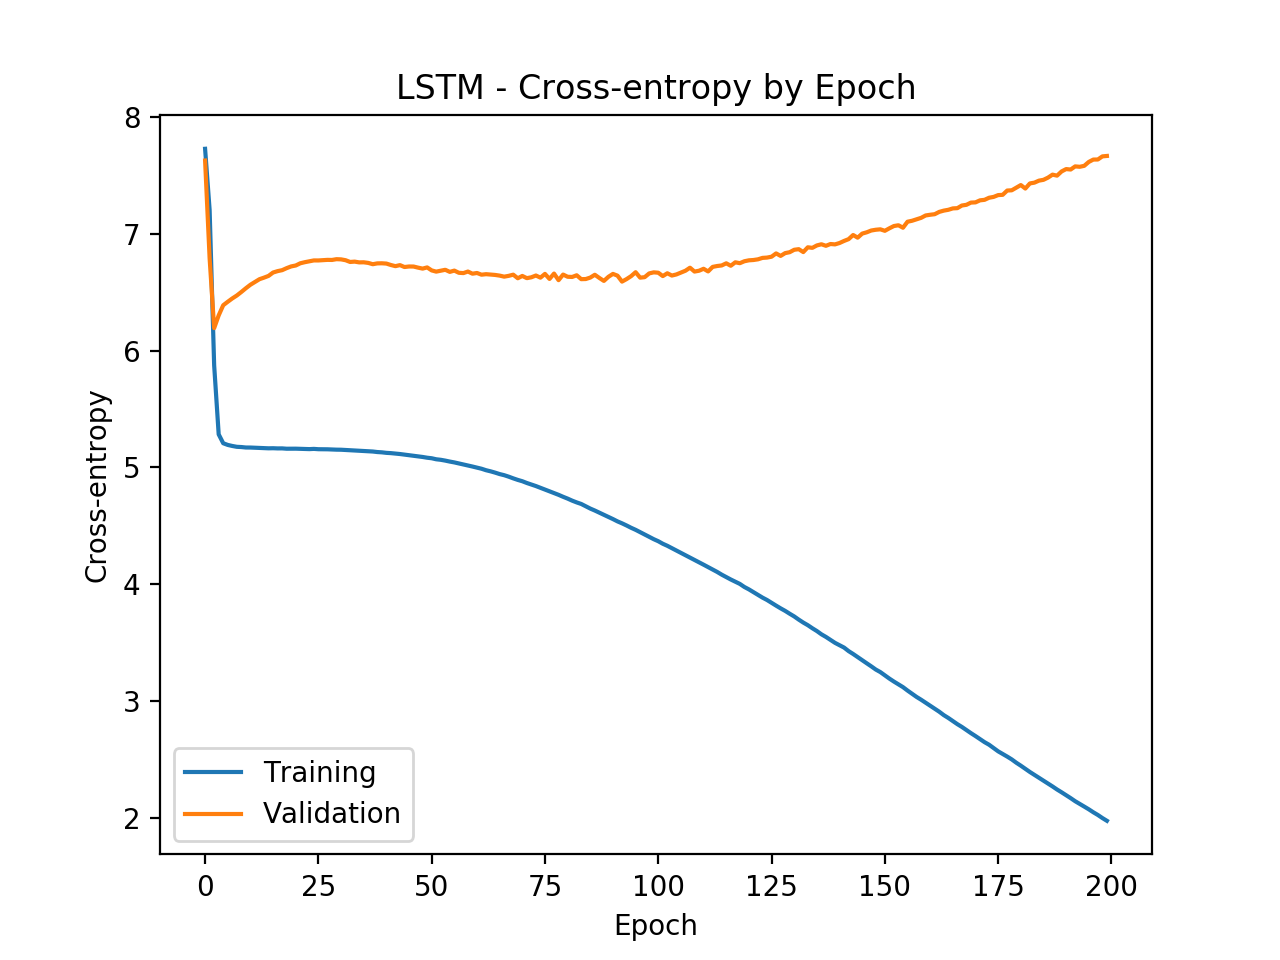
\includegraphics[width=0.42\textwidth]{LSTM_Loss.png}
    \caption{LSTM learning curves}
    \label{fig:LearningCurves}
\end{figure}

Section \ref{sec:discconclstm} contains an additional discussion on the LSTM model.

\subsubsection{Markov chain model}
\label{sec:markov}
Owing to the challenges in developing and training a successful neural sentence generator outlined in the previous section \ref{sec:lstm}, a model based on a popular open-source Markov chain library, \textit{markovify} \cite{markovify}, was implemented as the second generator of \textit{prose2poetry}.

A Markov chain is a statistical model which computes probabilities of sequences of random variables from a set of possible values, referred to as states \cite[Chapter~8]{jurafskymarkov}. They were first used by \citet{markov} to predict whether the next letter in a sequence was a vowel or a consonant. Figure \ref{fig:markov} shows a graphic of a Markov chain for English word transitions.

\begin{figure}
	\centering
	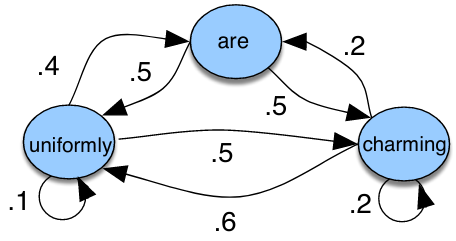
\includegraphics[scale=0.35]{./markov_chain.png}
	\caption{Illustration of Markov chain for word transition probabilities \cite{jurafskymarkov}}
\label{fig:markov}
\end{figure}

The Markov chain implementation in the \textit{markovify} library takes a corpus of sentences as an input, splits it into words, and builds probabilities of forward word transitions starting from the beginning of a sentence and moving towards the end. From this, new sentences can be generated using the observed word transition probabilities in the input corpus and a provided beginning word.

Additional work was done by \citet{markovifyfork} to implement a backwards Markov chain generator in the \textit{markovify} library. This reverses the order in which sentences from the corpus are consumed to build the model, resulting in word transitions that move backwards in a sentence starting from an ending word. This is exactly suitable for the purposes of \textit{prose2poetry}. The library also has checks to avoid exact recreations of the input text.

\subsubsection{Sentence semantic relatedness}
\label{sec:doc2vec}
As explained in section \ref{sec:fasttext}, the word pairs were selected to be related in context in the hopes that the two resulting generated sentences would be semantically related as well. An analysis was conducted to validate this assumption with the \textit{doc2vec} sentence embedding \cite{docvec}. The hyperparameters are shown in \ref{table:HP_fasttext}, and it was trained on the same input corpus.

For the Markov chain model, the cosine distance between the embedding vectors of two generated sentences showed an improvement of 10\% (evaluated across 1,000 generated couplets) when using end words that had a high FastText cosine distance. This justifies the design choice of ranking the generated rhyming word pairs by semantic similarity. The LSTM model saw an insignificant improvement of 0.6\%.

% Markov: 0.51799 vs 0.562932 
% LSTM: 0.607907 vs 0.611643

%%%%%%%%%%%%%%
% EXP & RESULTS		%
%%%%%%%%%%%%%%
\section{Experiments and Results}
\label{sec:results}

\subsection{Baseline corpora}
\label{sec:corpora}

Using a similar approach to \citet{cole}, the Gutenberg Poetry \cite{gutenbergpoetry} and PoetryFoundation \cite{poetryfoundationkaggle} datasets were filtered to produce rhyming couplets, as its easier to extract couplets from larger poetry datasets than it is to find datasets exclusively containing couplets.

The filtering process uses the rhymes function available in the pronouncingpy library to extract every pair with rhyming end words from the same poem as a couplet. The total is 331,713 rhyming couplets from Gutenberg, and 10,009 rhyming couplets from PoetryFoundation.

\subsection{Couplet evaluation}
\label{sec:coupleteval}

A couplet scoring function was developed to evaluate the couplets. The score focuses only on the form of the couplets. This is measured with two components -- the end word rhyme score, and a stress score which measures syllabic meter \cite{meter_def}.

\subsubsection{Rhyme score}
\label{sec:rhymescore}
The rhyme score returns a real value representing the strength of the rhyme between two words. It uses phoneme data from the CMUdict in a weighted sum of three heuristic scores:
\begin{tight_itemize}
	\vspace{-0.5em}
	\item \textit{Reverse consecutive phoneme matching} (RCPM):
	RCPM counts, in reverse order starting from the end of both words, how many consecutive phoneme matches occur between the two words, normalized by the maximum possible matches. Let $c^{(a,b)}_{\text{phoneme}}$ be the reverse consecutive phoneme matches between words $a$ and $b$ and let $n^{(i)}_{\text{phoneme}}, i = {a, b}$ be the phoneme count for the words $a$ and $b$, then:
	$$\textrm{RCPM}^{(a,b)} = \frac{c^{(a,b)}_{\text{phoneme}}}{\min(n^{(a)}_{\text{phoneme}}, n^{(b)}_{\text{phoneme}})}$$
	\item \textit{Overall phoneme matching} (OPM):
		OPM counts all common phonemes between a pair of words without considering order. Let $m^{(a,b)}_{\text{phoneme}}$ be the total number of phoneme matches between word $a$ and $b$, and $n^{(i)}_{\text{phoneme}}, i = {a, b}$ be the phoneme counts for words $a$ and $b$, then:
		$$\textrm{OPM}^{(a,b)} = \frac{2 * m^{(a,b)}_{\text{phoneme}}}{n^{(a)}_{\text{phoneme}} + n^{(b)}_{\text{phoneme}}}$$
		This can be considered an adapted \citet{ratcliff} string similarity score with phonemes instead of characters.
	\item \textit{Syllable count matching} (SCM):
	The last score selects for words close in number of syllables. Let $n^{(i)}_{\text{syllable}}, i = {a, b}$ be the total counts of syllables in words $a$ and $b$.
	\begin{equation}
	\textrm{SCM}^{(a,b)} = 
	\begin{cases}
	\nonumber 1 \text{ if $\max(n^{(a)}_{\text{syllable}}, n^{(b)}_{\text{syllable}})$ = 1}\\
	\nonumber \frac{\min(n^{(a)}_{\text{syllable}}, n^{(b)}_{\text{syllable}}) - 1}{\max(n^{(a)}_{\text{syllable}}, n^{(b)}_{\text{syllable}}) - 1} \text{ otherwise}\\
        \end{cases}
	\end{equation}
	The subtraction by 1 is to ensure that the lowest possible SCM score can be 0.
\end{tight_itemize}

These are combined in an evenly weighted average. Examples of rhyme scores are shown in the code example in figure \ref{fig:rhymescorecode}. There are some additions for special cases:
\begin{tight_enumerate}
	\vspace{-0.5em}
	\item
		Identical words have a rhyme score of 0.
	\item
		Longer rhymes score higher, up to a ceiling of 6 phonemes. Without this, single-syllable words tend to dominate the rhyme score.
	\item
		If there are multiple possible pronunciations, rhyme score returns the maximum score across all the pronunciation permutations for word $a$ and $b$, discussed further in section \ref{sec:synset}.
\end{tight_enumerate}

\begin{figure}
\begin{Verbatim}[fontsize=\small]
>>> rhyme_score('affection', 'perfection')
0.88
>>> rhyme_score('affection', 'disgust')
0.075
\end{Verbatim}
\caption{Some examples of rhyme score}
\label{fig:rhymescorecode}
\end{figure}

\subsubsection{Meter score}
\label{sec:stressscore}

Using the pronouncingpy library, the syllabic stress of all of the words in each line is concatenated to represent the syllabic meter \cite{meter_def} of each sentence. In the CMUdict, 0 represents an unstressed syllable, 1 represents primary stress, and 2 represents secondary stress.  Examples are shown in table \ref{table:stress}. The \citet{ratcliff} string similarity score is then applied on the concatenated stress strings of the two sentences in the couplet.

\begin{table}
\centering
\begin{tabular}{ll c c}
	\hline\hline
	Sentence & Stress \\ [0.5ex]
	\hline\hline
	He likes jam & 111 \\ [0.5ex]
	\hline
	She likes ham & 111 \\ [0.5ex]
	\hline
	Alexander the Great conquered & 20100110 \\ [0.5ex]
	\hline
\end{tabular}
\caption{Cases of matched and mismatched stress strings for comparing meter}
\label{table:stress}
\end{table}

\subsubsection{Couplet score}
\label{sec:coupletscore}

The total couplet score is an evenly weighted sum of the two metrics above, resulting in a single real value $\in [0, 1]$.
 It was mentioned that the couplet score is focused on form only, and not couplet contents. This can be problematic -- consider the example ``ham ham ham, jam jam jam.'' This couplet has a nearly perfect score of 0.89 (out of 1.0) since it rhymes and has exactly matching meter. However, a human judge wouldn't rate it as good poetry. There were many challenges involved in evaluating the semantic coherence, grammatical correctness, or other aspects of the contents of the couplets. These are discussed in section \ref{sec:nlg}.

\begin{table*}[ht]
\begin{tabular}{|l|l|l|l|l|l|l|l|l|l|l|c|c|c|c|c|c|c|c|c|c|}
\hline\hline
\multicolumn{1}{|c|}{Score} & \multicolumn{3}{c|}{Couplet} & \multicolumn{3}{c|}{Rhyme} & \multicolumn{3}{c|}{Meter}\\
\cline{1-10}
\multicolumn{1}{|c|}{Dataset} & Mean & SD & .95q & Mean & SD & .95q & Mean & SD & .95q \\
\hline\hline
Gutenberg & 0.69 & 0.12 & 0.86 & 0.70 & 0.18 & 0.93 & 0.68 & 0.14 & 0.89 \\ [0.5ex]
\hline
PoetryFoundation & 0.68 & 0.12 & 0.85 & 0.70 & 0.19 & 0.93 & 0.68 & 0.14 & 0.89 \\ [0.5ex]
\hline
\textit{prose2poetry} LSTM & 0.59 & 0.12 & 0.78 & 0.68 & 0.17 & 0.91 & 0.50 & 0.19 & 0.80 \\ [0.5ex]
\hline
\textit{prose2poetry} Markov chain & 0.58 & 0.12 & 0.77 & 0.68 & 0.17 & 0.90 & 0.47 & 0.19 & 0.77 \\ [0.5ex]
\hline
Prose & 0.33 & 0.13 & 0.56 & 0.19 & 0.18 & 0.46 & 0.48 & 0.19 & 0.76 \\ [0.5ex]
\hline
\end{tabular}

\caption{Couplet scores of \textit{prose2poetry} generated outputs and baselines}
\label{table:couplet_results}
\end{table*}

\begin{table*}[ht]
\begin{tabular*}{\textwidth}{ll cc}
	\hline\hline
	Source & Couplet \\ [0.5ex]
	\hline\hline
	Gutenberg baseline & (`The vision came and went', `The light shone and was spent') \\ [0.5ex]
	\hline
	PoetryFoundation baseline & (`Tells himself that he tried', `Tells himself that he cried and cried') \\ [0.5ex]
	\hline
	Prose & (`the mistake had been slight', `the carriage was sent for them now') \\ [0.5ex]
	\hline
	\textit{prose2poetry} LSTM & (`had her neighborhood drinking', `though her sinking' \\ [0.5ex]
	\hline
	\textit{prose2poetry} Markov chain & (`I could never see a better', `I hope , a highly prized letter') \\ [0.5ex]
	\hline
\end{tabular*}
\caption{Examples of top-scoring couplets from all evaluated datasets}
\label{table:bestcouplets}
\end{table*}

\subsection{Results}
\label{sec:results}
\subsubsection{Quantitative assessment}

The results in table \ref{table:couplet_results} were evaluated on 1,000 couplets randomly selected from the baselines and \textit{prose2poetry} generator models. These were selected to be a representative sample from the larger datasets. The evaluation was repeated with different RNG seeds, observing that different random selections of couplets from the same source tended to have a stable score.

The prose baseline was created by selecting random sentence pairs from the input English novel corpus without any filtering. The total couplet score is shown, as well as each of the subcomponents for further discussion. The mean, standard deviation, and .95 quantile were chosen as statistical metrics.

\subsubsection{Qualitative assessment}

From each evaluated dataset, one couplet which scored better than the .95 quantile score is included in table \ref{table:bestcouplets} for the readers to enjoy and judge for themselves.

%%%%%%%%%%%%%%
% DISC & CONC		%
%%%%%%%%%%%%%%
\section{Discussion and conclusion}
\label{sec:discconc}

\textcolor{green}{
Results interpretation here. "Our poems scored well, stress score showed real poems have good meter, etc."
}

\textcolor{Orchid}{
\subsection{Sevag discussion/conclusion ideas}
sevag ideas
}

\subsection{LSTM model discussion}
\label{sec:discconclstm}

The trained LSTM described in section \ref{sec:lstm} did not perform to the expected standard. Using additional input corpora would have been against the spirit of \textit{prose2poetry}, so it was discarded as an option. One possible alternative could have been to use a pre-trained language model such as GPT-2 \cite{gpt2}, fine-tuned with the input prose corpus.

\subsection{Multiple pronunciations and sense disambiguation}
\label{sec:synset}

Difficulty was encountered in the rhyme score when trying to associate different pronunciations of homographs with their respective senses or parts of speech. \citet{hopkins-kiela-2017} encountered the same difficulty. Consider two examples, using WordNet \cite{wordnet} as a lexical resource:
\begin{tight_enumerate}
	\vspace{-0.5em}
	\item
		In the CMUdict, there are two pronunciations for ``bow'': like ``cow'' or like ``snow''. In WordNet, there are fourteen synsets for ``bow'', and two different parts of speech.
	\item
		In the CMUdict, there are two pronuncations for ``defect'': noun with beginning emphasis ``DEE-fect'', or verb with end emphasis ``de-FECT''. In WordNet, there are five synsets for ``defect'', and two different parts of speech.
\end{tight_enumerate}

There is no readily available mapping between CMUdict pronunciation and WordNet senses. This can only be resolved with a lexical resource that provides combined sense and pronunciation disambiguation -- Wiktionary \cite{wiktionary} is one such option, but scraping it was considered beyond the scope of this paper. The final approach chosen was to ignore ambiguity and return the best rhyme score across all possible pronunciation permutations.

\subsection{Sentence content evaluation}
\label{sec:nlg}

The biggest difficulty encountered in \textit{prose2poetry} was finding a way to quantitatively evaluate the contents of the couplet. Throughout the development of the couplet scoring function, this was narrowed down to two major criteria -- are the two sentences related semantically, and are the two sentences grammatically correct. The latter is especially tricky with poetry, which does not necessarily need to strictly obey grammar. Semantic relatedness was covered in section \ref{sec:doc2vec}.

The field of NLG (Natural Language Generation) evaluation was explored for ideas to evaluate grammatical correctness. \citet{nlgeval} present a survey on popular automated metrics for evaluating machine-generated text in several applications including machine translation and dialogue response systems. They found that METEOR \cite{meteor} correlates well at the sentence level with human judgement.

An important requirement of automated NLG evaluation metrics reference sentences to compare the inputs to. When scoring poetry, it is unclear what the references should be. In an early experiment, the baseline couplets from the Gutenberg poetry corpus were used as reference sentences in METEOR. It was hoped that this would score generated couplets high if they resembled good poetry. This did not work -- in practice, the METEOR scores were found to be inappropriate for this task, and they could not distinguish human-judged bad and good sentences.

\textcolor{Orchid}{
\subsection{Code availability}
Describe open source code location, GitHub link, package structure (very brief), etc.
}

%%%%%%%%%%%%%%
% STAT OF CONT		%
%%%%%%%%%%%%%%
\section{Statement of contributions}
\label{sec:contributions}
Sevag Hanssian worked on finding different poem baselines \& the prose dataset, creating the coding architecture, developing the couplet scoring and running the experiments. François Milot developed the word embedding (FastText), the doc2vec training, the word pair generation and design of the rhyme score. Also, the design and direction of the project have been decided as a group. 

\bibliographystyle{acl_natbib}
\bibliography{final_report}

\end{document}
